\chapter{Visualizing the source density phase space}
With the measurement of a diffuse neutrino flux but uncertainties in the astrophysical origins, one can ask if the dominant source class which produces neutrinos are \textit{rare and bright} or \textit{numerous and dim}. One way to do this is by looking for point source excesses. With the lack of any clear point sources, neutrino bright objects can be excluded, and thus attributing the entire diffuse flux from steady, rare ($<\mathcal{O}(1\; \mathrm{Gpc}^{-3})$) objects can be excluded with current limits. The effective source densities which can be probed change significantly with a detector like Gen2. All of this is normally visualized in Figure~\ref{fig:current_fig} (Figure taken from \cite{Aartsen:2019swn}).

\begin{figure}[h!]
    \centering
    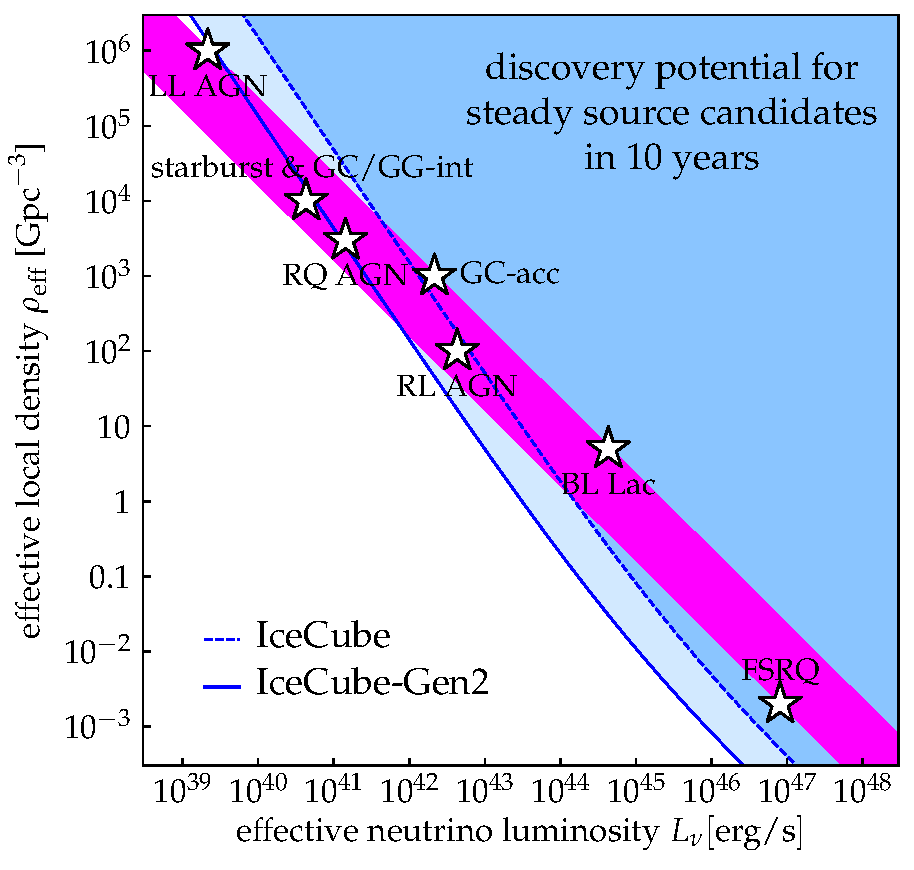
\includegraphics[width=0.45\textwidth]{images/continuous_Gen2_revised.pdf}
    \caption{Comparison of the diffuse neutrino flux (magenta) to current and projected point source sensitivities (blue lines), as well as the effective local source density and luminosity of various candidate source classes.}
    \label{fig:current_fig}
\end{figure}

A quick notes about the figure: making an argument such as ``x\% of source class y could still explain the diffuse flux'' is true if the star corresponding to source class y, when moved down on the y-axis by the appropriate ratio, is below the point source limits.

This way of visualizing the parameter space downplays the large region of parameter space the Gen2 could probe. Also, it is the transpose of what you might intuitively do, as luminosity is somewhat analagous to flux, which we plot vertically and forbid regions above (not to the right of) limits. Additionally, even under the assumption that numerous source classes contribute to the diffuse flux, there are likely only one or a few that contribute at a greater than 10\% level, and these are the real targets of searches in this spirit. As a result, the true parameter space of interest is not as large as this plot would lead you to believe. 

Some suggestions for improvement include transposing the plot and possibly hatching the part of the parameter space that explains 100\% of the diffuse flux once we have gen2, as is pictured in Figure~\ref{fig:transposed}.

\begin{figure}[htb]
    \centering
    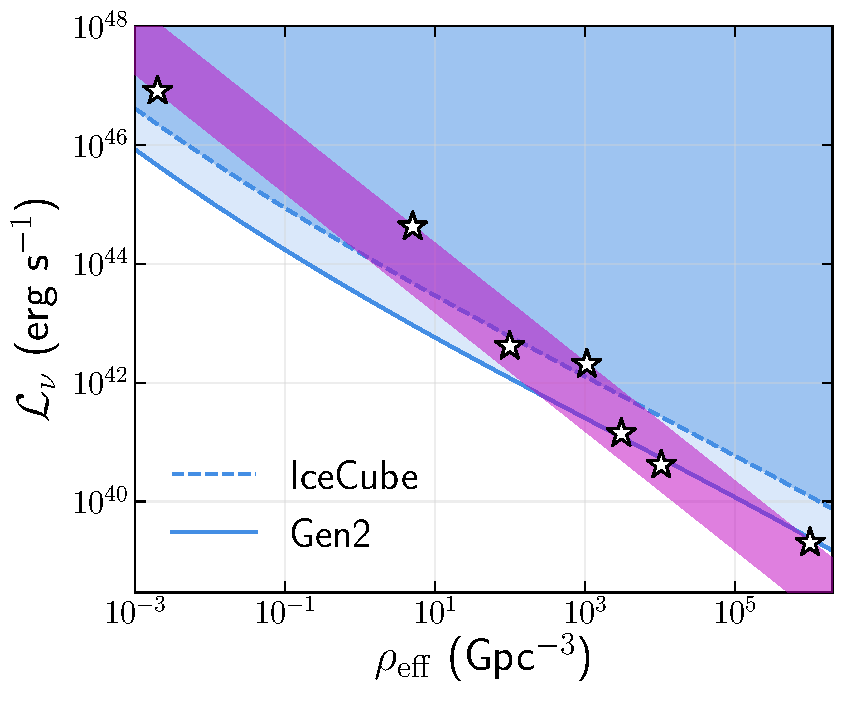
\includegraphics[width=0.48\textwidth]{images/lumi_density_rotated.pdf}
    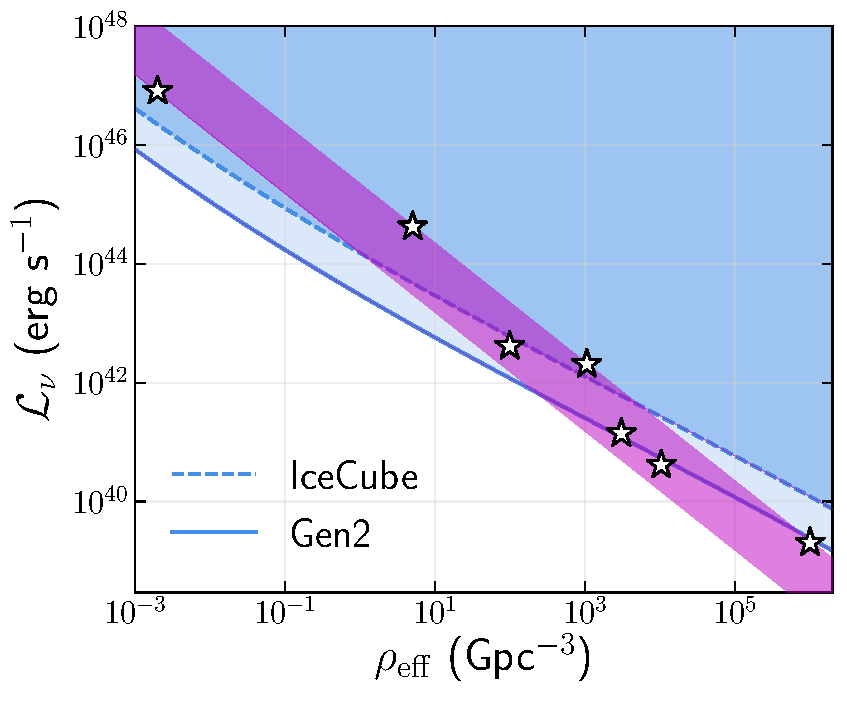
\includegraphics[width=0.48\textwidth]{images/lumi_density_hatched_rotated.pdf}
    \caption{Transpose of the previous figure, so that higher luminosities are found by moving vertically upwards in the plot}
    \label{fig:transposed}
\end{figure}

This plot still has the problem of presenting a lot of uninteresting phase space (bottom left). To remedy this, we could plot $\rho_{eff}\times \mathcal{L}_{\nu}$ on the vertical axis, in much the same way that power law spectra are scaled by powers of $E_{\nu}$. Doing this results in Figure~\ref{fig:scaled_lumi_density}.

\begin{figure}
    \centering
    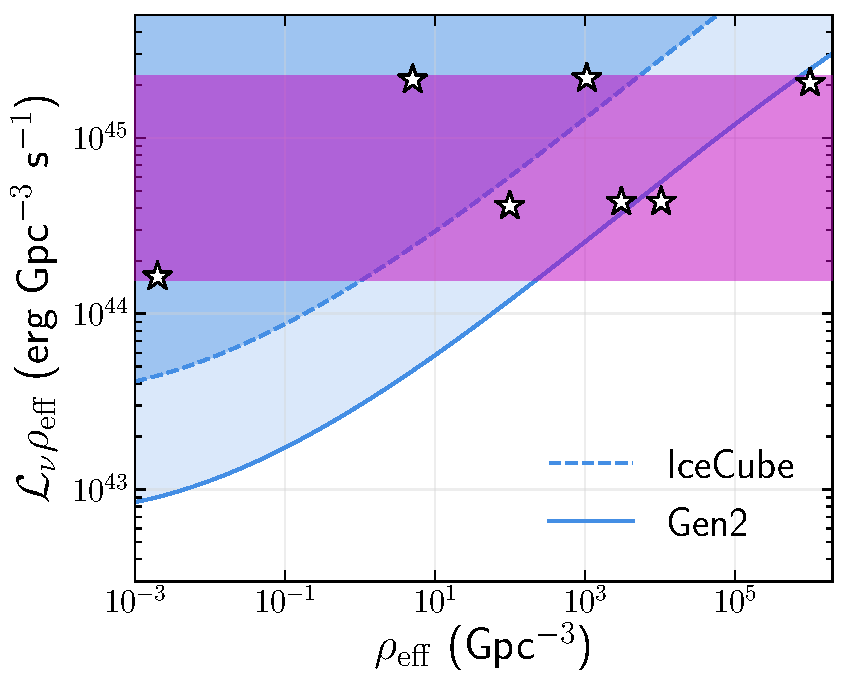
\includegraphics[width=0.48\textwidth]{images/lumi_density_product.pdf}
    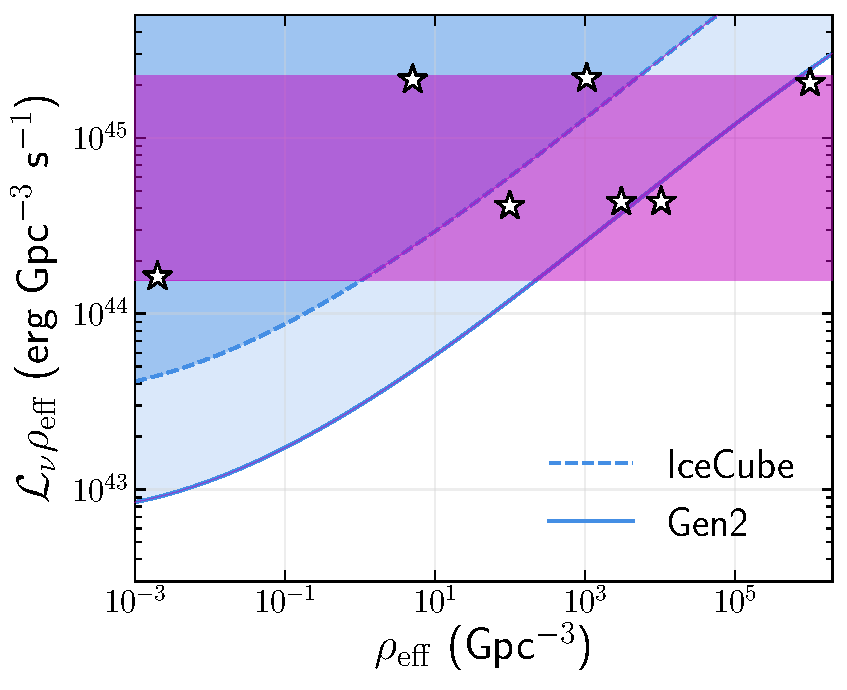
\includegraphics[width=0.48\textwidth]{images/lumi_density_product_hatch.pdf}
    \caption{Luminosity times effective local density plotted on the y-axis to focus on the interesting region of parameter space.}
    \label{fig:scaled_lumi_density}
\end{figure}

One nice consequence of this visualization is suppose you have a candidate source class that could produce a fraction, $f$ of the diffuse flux. Then (ignoring uncertainties on the diffuse flux), this just corresponds to moving down in the plot by a factor of $f$ from the vertical magenta line. This is shown in Figure~\ref{fig:diffuse_fraction_lumi}. 

\begin{figure}[h!]
    \centering
    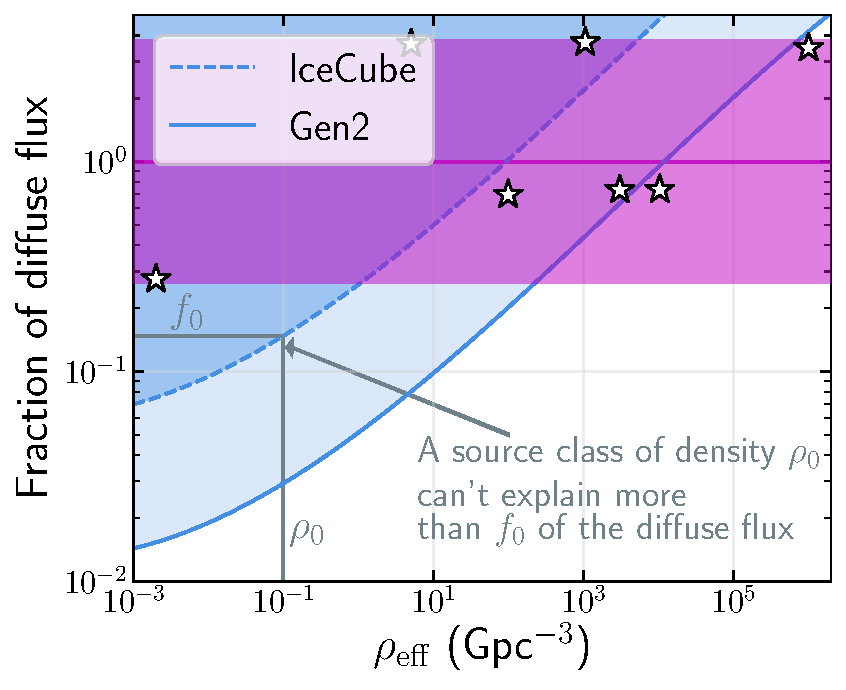
\includegraphics[width=0.5\textwidth]{images/lumi_density_fraction.pdf}
    \caption{Similar figure as above, scaled by the diffuse flux to highlight interpretation.}
    \label{fig:diffuse_fraction_lumi}
\end{figure} 